\documentclass[conference,letterpaper]{IEEEtran}
\usepackage{amsmath}

\usepackage{graphicx}
\usepackage{subcaption}
\usepackage{fixltx2e}
\usepackage{gensymb}
\usepackage{todonotes}
\usepackage{url}
\usepackage{float}
\usepackage{hyperref}


% correct bad hyphenation here

\hyphenation{op-tical net-works semi-conduc-tor top-ology}
\setlength {\marginparwidth }{2cm}

\begin{document}

%%%%%%%%%%%%%%%%%%%%%%%%%%%%%%%%%%%%
% paper title
%%%%%%%%%%%%%%%%%%%%%%%%%%%%%%%%%%%%
% can use linebreaks \\ within to get better formatting as desired
\title{XAI-Driven TinyML with Compact Models for Compromised IoT Device Detection}
%%%%%%%%%%%%%%%%%%%%%%%%%%%%%%%%%%%%
% author names and affiliations
%%%%%%%%%%%%%%%%%%%%%%%%%%%%%%%%%%%%
% option 1)
%%%%%%%%%%%%%%%%%%%%%%%%%%%%%%%%%%%%
% use a multiple column layout for up to three different
% affiliations


% \IEEEauthorblockN{More authors}
% \IEEEauthorblockA{Starfleet Academy\\
% San Francisco, California 96678-2391}
% }

% for over three affiliations, or if they all won't fit within the width
% of the page, use this alternative format:

%%%%%%%%%%%%%%%%%%%%%%%%%%%%%%%%%%%%
% option 2)
%%%%%%%%%%%%%%%%%%%%%%%%%%%%%%%%%%%%
\author{\IEEEauthorblockN{Bodapatla Rakesh}
\IEEEauthorblockA{Indian Institute of Information Technology and Management \\ Gwalior \\ 2021IMT-022 }
\\
\IEEEauthorblockN{Gulla Akshaya}
\IEEEauthorblockA{Indian Institute of Information Technology and Management \\ Gwalior \\ 2021IMT-038 }
\\
\IEEEauthorblockN{NVNL Ishwarya}
\IEEEauthorblockA{Indian Institute of Information Technology and Management \\ Gwalior \\ 2021IMT-070 }
\\
\IEEEauthorblockN{Vennapusa Ramana Reddy}
\IEEEauthorblockA{Indian Institute of Information Technology and Management \\ Gwalior \\ 2021IMT-110 }
}


%%%%%%%%%%%%%%%%%%%%%%%%%%%%%%%%%%%%
% make the title area
%%%%%%%%%%%%%%%%%%%%%%%%%%%%%%%%%%%%
\maketitle
\thispagestyle{plain}
\pagestyle{plain}

%%%%%%%%%%%%%%%%%%%%%%%%%%%%%%%%%%%%
% Abstract
%%%%%%%%%%%%%%%%%%%%%%%%%%%%%%%%%%%%
\begin{abstract}
%\boldmath
The growing adoption of Internet of Things (IoT) devices has introduced critical challenges in ensuring their security, especially given their deployment in resource-constrained environments. Traditional Machine Learning (ML) solutions, though effective, are often too computationally intensive for direct deployment on IoT end devices. This research explores the use of Tiny Machine Learning (TinyML) techniques augmented with Explainable AI (XAI) to detect compromised IoT devices with high accuracy and low resource overhead. Leveraging a subset of the IoT23 dataset, our study focuses on model optimization through techniques like quantization and knowledge distillation, significantly reducing model size while maintaining performance. Furthermore, SHAP and LIME are employed to provide interpretability by identifying impactful features, ensuring transparency in predictions. Experimental simulations on devices like Raspberry Pi 4 and Arduino Nano 33 BLE Sense demonstrate the feasibility of deploying compact ML models in real-world IoT settings. Our findings contribute to the development of energy-efficient, interpretable, and deployment-ready ML models, enabling secure and intelligent monitoring across IoT ecosystems.
\end{abstract}
% IEEEtran.cls defaults to using nonbold math in the Abstract.
% This preserves the distinction between vectors and scalars. However,
% if the conference you are submitting to favors bold math in the abstract,
% then you can use LaTeX's standard command \boldmath at the very start
% of the abstract to achieve this. Many IEEE journals/conferences frown on
% math in the abstract anyway.

% no keywords

% For peer review papers, you can put extra information on the cover
% page as needed:
% \ifCLASSOPTIONpeerreview
% \begin{center} \bfseries EDICS Category: 3-BBND \end{center}
% \fi
%
% For peerreview papers, this IEEEtran command inserts a page break and
% creates the second title. It will be ignored for other modes.
\IEEEpeerreviewmaketitle


%%%%%%%%%%%%%%%%%%%%%%%%%%%%%%%%%%%%%%%%%%%%%%%%%%%%%%%%%%%%%%%%%%%%%%
%% INTRODUCTION
%%%%%%%%%%%%%%%%%%%%%%%%%%%%%%%%%%%%%%%%%%%%%%%%%%%%%%%%%%%%%%%%%%%%%%
\section{Introduction}
\subsection{Internet of Things}
The Internet of Things (IoT) has revolutionized the way we interact with the world around us. It encompasses a vast network of interconnected devices, ranging from everyday appliances like smart thermostats and voice assistants to industrial sensors and complex medical equipment. These devices collect and exchange data, enabling automation, remote monitoring, and enhanced functionality across various sectors.
~\\
~\\
The applications of IoT are widespread and continuously evolving. In smart homes, thermostats adjust to our preferences, refrigerators monitor food supplies, and security systems provide real-time alerts. Smart cities leverage connected sensors for traffic management, waste collection optimization, and environmental monitoring. The healthcare industry utilizes wearable devices for patient health tracking and remote monitoring, while industrial applications employ IoT sensors for predictive maintenance and improved operational efficiency.
~\\
~\\
Despite the undeniable benefits, the expanding IoT landscape presents a growing concern: security vulnerabilities. Due to their inherent resource limitations and focus on functionality, many IoT devices lack robust security protocols. This makes them prime targets for cyberattacks, potentially compromising data privacy, disrupting critical operations, and even causing physical harm. Attackers can exploit these vulnerabilities to gain unauthorized access, steal sensitive data, or disrupt device functionality. Malicious actors can also leverage compromised IoT devices to launch large-scale attacks on networks and critical infrastructure.
~\\
~\\
This research focuses on improving the security of IoT devices by making machine learning models smaller, faster, and easier to understand. We investigate how lightweight ML models can be used to detect if an IoT device has been compromised, while also ensuring the model can run directly on edge devices with limited resources. By using techniques like Knowledge Distillation and Explainable AI, we aim to build compact models that not only perform well but also explain their predictions clearly. This helps in making real-time decisions while saving energy and increasing trust in automated systems.

\subsection{Intrusion Detection Systems}
Intrusion Detection Systems (IDS) act as a vigilant guardian within network security ecosystems.  These systems function by continuously monitoring network traffic and system activity, searching for any signs of malicious intent or policy violations. Through meticulous analysis of network packets, system logs, and other data sources, IDSs can pinpoint suspicious patterns or behaviors that may signal an ongoing attack.
~\\
~\\
There are two main classifications of IDSs, distinguished by their deployment strategy:
\\
\subsubsection{Network-based Intrusion Detection Systems (NIDS)}\\ These systems function as watchful sentinels on network segments or at the network perimeter, meticulously examining network traffic flowing across those points.  NIDS meticulously analyze network packets for known attack signatures, anomalies in traffic patterns, or content that transgresses security policies.

\subsubsection{Host-based Intrusion Detection Systems (HIDS)}\\ As the name implies, HIDS reside on individual devices within a network, acting as vigilant guards on those specific systems.  They monitor system activity for any suspicious events, unauthorized access attempts, or modifications to critical system files.  HIDS are particularly adept at detecting insider threats or attacks that have infiltrated past perimeter defenses.
~\\
~\\
The advantages of IDSs are undeniable. They function as an early warning system, providing security teams with a critical head start in detecting ongoing attacks. This allows for swift action to mitigate potential damage. Additionally, IDSs offer valuable insights into network traffic patterns and potential threats, empowering security teams to prioritize their response efforts and allocate resources effectively. Furthermore, the presence of an IDS can act as a psychological deterrent, reminding attackers that their actions are under constant scrutiny.
~\\
~\\
However, IDSs also have limitations.  One challenge is the potential for false positives.  Overly cautious IDSs can generate alerts for harmless activity, leading to alert fatigue for security personnel and potentially delaying the identification of genuine threats.  Another challenge is the ever-evolving threat landscape.  Attackers are constantly developing new tactics and techniques to evade detection.  Consequently, IDSs require regular updates to maintain effectiveness against the latest threats.  Finally, while some advanced IDSs can take automated actions to isolate compromised systems, most rely on security personnel to investigate and respond to detected threats.
~\\
~\\
As IoT devices become more widespread, traditional IDS solutions struggle with resource limitations and lack of interpretability. This project addresses those challenges by combining Explainable AI (XAI) with TinyML to build lightweight, interpretable intrusion detection models. Using techniques like LIME, SHAP, quantization, and knowledge distillation, we create compact models that can run efficiently on edge devices like Raspberry Pi and Arduino Nano—ensuring real-time security without sacrificing transparency or performance.

\subsection{Role of TinyML and Explainable AI in IoT Intrusion Detection}
Role of TinyML and Explainable AI in IoT Intrusion Detection
Tiny Machine Learning (TinyML) and Explainable Artificial Intelligence (XAI) offer a powerful solution to the limitations of traditional IDS in IoT environments. IoT devices, often constrained by limited memory, processing power, and energy, require models that are both efficient and lightweight. TinyML addresses this by enabling the deployment of compact machine learning models directly on edge devices, reducing reliance on cloud resources and ensuring real-time responses. At the same time, XAI techniques such as LIME and SHAP provide interpretability, allowing security analysts and system developers to understand why a model flags a device as compromised which is crucial for trust and accountability in security applications.
~\\
There are several ways this integrated approach enhances IDS for IoT:
~\\
\subsubsection{Efficient Anomaly Detection}: TinyML enables models to detect behavioral deviations in real-time, directly on the device, without cloud latency or power drain.
~\\
\subsubsection {Transparent Classification}: With XAI, even lightweight models can offer explanations for their classifications, helping to identify the features that triggered a threat label.
~\\
\subsubsection {Model Optimization}: Techniques like quantization and knowledge distillation reduce model complexity and size, making them ideal for microcontroller-class devices.
~\\

Together, TinyML and XAI form a robust, interpretable, and scalable foundation for modern intrusion detection systems in IoT networks—offering both performance and transparency without compromising on resource efficiency.
%%%%%%%%%%%%%%%%%%%%%%%%%%%%%%%%%%%%%%%%%%%%%%%%%%%%%%%%%%%%%%%%%%%%%%
%% NEW SECTION HEADER
%%%%%%%%%%%%%%%%%%%%%%%%%%%%%%%%%%%%%%%%%%%%%%%%%%%%%%%%%%%%%%%%%%%%%%
\section{Past Work}
 The Problem of Intrusion using IOT 23 Dataset was previously worked upon by Cruz et al.\cite{9831021}.
Their Paper used only XGBoost to perform a task of Binary classification. This has ignored the nuances that such a Multiclass Data Represents. The Proposed model could be optimized further by taking this into account. Furthermore, their paper was limited to only one model. Multiple models would prove to be more useful in such tasks. 

Another significant work is by Tekin et al.\cite{basepaper2}, who analysed energy consumption of on-device machine learning models for IoT intrusion detection. Their study examined key factors such as model inference time, training time, power consumption, and energy efficiency. However, their work has certain limitations. In practice, when the model size is several MB's, quantization methods may not prove to be effective due to the potential loss in model accuracy. To overcome these shortcomings, we propose utilizing knowledge distillation as an alternative approach, which can significantly reduce the model size while retaining its performance.




%%%%%%%%%%%%%%%%%%%%%%%%%%%%%%%%%%%%%%%%%%%%%%%%%%%%%%%%%%%%%%%%%%%%%%
%% NEW SECTION HEADER
%%%%%%%%%%%%%%%%%%%%%%%%%%%%%%%%%%%%%%%%%%%%%%%%%%%%%%%%%%%%%%%%%%%%%%
\section{The Datset}

The dataset chosen for this research is the famous, IoT23 Dataset.

IoT-23 introduces a novel dataset comprising network traffic data emanating from Internet of Things (IoT) devices. The dataset encompasses 20 instances of malware activity observed in IoT devices, alongside 3 instances of benign IoT device traffic. Its primary objective is to furnish researchers with a substantial dataset containing labeled instances of both IoT malware infections and benign IoT traffic, facilitating the development of machine learning algorithms. Each of the twenty-three captures, referred to as scenarios, represents distinct IoT network traffic behaviours. In malicious scenarios, specific malware samples were executed on Raspberry Pi devices, utilizing various protocols and executing diverse actions. Conversely, benign scenarios involved capturing network traffic from actual IoT devices, including a Philips HUE smart LED lamp, an Amazon Echo home intelligent personal assistant, and a Somfy smart door lock. Notably, these IoT devices are authentic hardware, not simulations, enabling the capture and analysis of real network behavior.

% ------------------------------------------------
% FIGURE: Frog
% ------------------------------------------------
\begin{figure}[hbt!] 
\centering
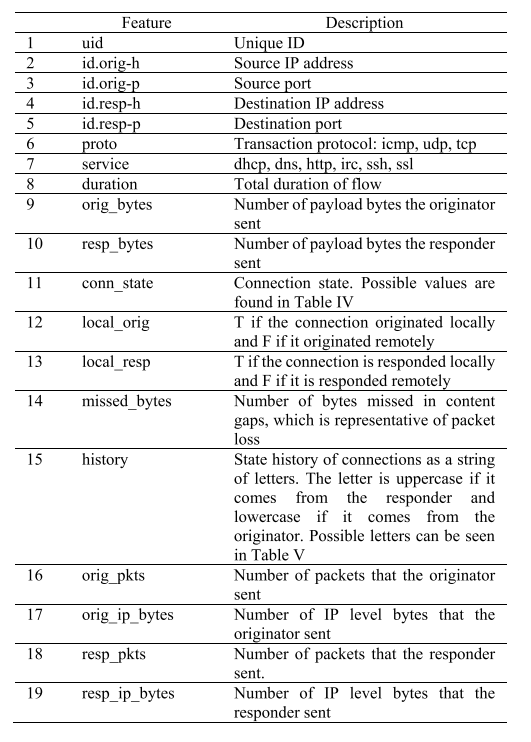
\includegraphics[width=0.46\textwidth]{figures/Features table}
\caption{Features and their descriptions.}
\label{fig:feat}
\end{figure}

% \begin{figure}[hbt!] 
% \centering
% 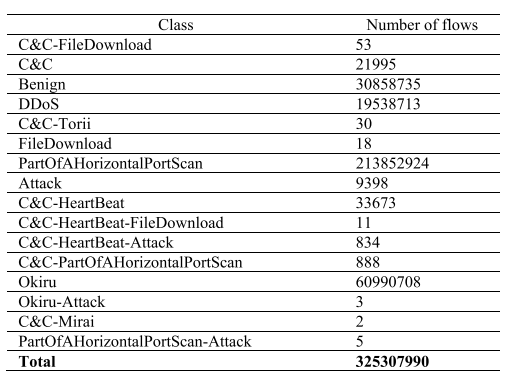
\includegraphics[width=0.46\textwidth]{figures/Labels}
% \caption{Class Labels.}
% \label{fig:feat}
% \end{figure}

%%%%%%%%%%%%%%%%%%%%%%%%%%%%%%%%%%%%%%%%%%%%%%%%%%%%%%%%%%%%%%%%%%%%%%
%% Summary
%%%%%%%%%%%%%%%%%%%%%%%%%%%%%%%%%%%%%%%%%%%%%%%%%%%%%%%%%%%%%%%%%%%%%%
\section{Data Preprocessing}
The features 'local\_orig' and 'local\_resp' were empty across all files, leading to their removal. Following established practices in pre-processing intrusion detection datasets, features containing IP addresses and port numbers were also discarded. Additionally, the 'history' feature, representing a sequence of connection values, was initially excluded. The correlation graph revealed a strong correlation between 'orig\_pkts' and 'orig\_ip\_bytes', as well as 'resp\_pkts' and 'resp\_ip\_bytes', resulting in the removal of the latter correlated features. Extreme minority classes containing fewer than 100 samples, such as 'C\&C-FileDownload' and 'FileDownload', were eliminated. Null values within various features were eliminated. Categorical features like 'service', 'proto', and 'conn\_state' underwent one-hot encoding, a common technique in previous studies, followed by normalization between 0 and 1 using min-max scaling.


% conference papers do not normally have an appendix

\section{Feature Selection using XAI}
Explainable Artificial Intelligence (XAI) is all about making AI systems more transparent and understandable to humans. As AI becomes more integrated into critical areas like healthcare, finance, and law, it's no longer enough for a model to simply give accurate results—it must also be able to explain how and why it arrived at those results. XAI helps bridge the gap between complex machine learning models and human reasoning by offering insights into the decision-making process, highlighting which features were most influential or what patterns the model recognized. This not only builds trust but also allows users to detect potential biases or errors, making AI systems more reliable and accountable.
\subsection*{Local and Global Explanations in XAI}

In Explainable Artificial Intelligence (XAI), we often talk about two types of explanations: {local} and {global}. These help us understand how an AI model makes decisions.

{Local explanations} focus on a single prediction. They help us understand why the model gave a certain result for one specific input. For example, if an AI model predicts that a person should not get a loan, a local explanation can show which features (like income, credit score, or debt) influenced that decision. Methods like \textit{LIME} were used for Local Explanations and \textit{SHAP} was used for global explanations.

{Global explanations}, on the other hand, give us an overall view of how the model works with the entire dataset. They help answer questions like: Which features are most important in general? What patterns does the model follow when making predictions? Global explanations are useful for understanding the model’s general behavior and making sure it is fair and reliable.

We have utilised global explanations to select most relevant and important features for the models. 
\subsection*{LIME: Local Interpretable Model-Agnostic Explanations}

LIME is a technique designed to explain the predictions of any machine learning model by learning an interpretable model locally around the prediction. Instead of trying to understand the entire model (which might be complex and non-linear), LIME focuses on explaining individual predictions using a simple, interpretable model like a linear model or a decision tree.

Let \( f: \mathbb{R}^d \rightarrow \mathbb{R} \) be the original complex model that we want to explain. Given a data instance \( x \in \mathbb{R}^d \), LIME tries to approximate \( f \) locally around \( x \) using an interpretable model \( g \) (such as a linear model).

\subsubsection*{Mathematical Formulation}

To approximate the original model \( f \) around an instance \( x \), LIME perturbs the input \( x \) to generate a set of synthetic data points \( \{ z_i \}_{i=1}^N \). For each perturbed sample \( z_i \), we obtain the prediction \( f(z_i) \) from the original model.

A proximity measure \( \pi_x(z) \) is used to assign weights to the perturbed samples based on how close they are to the original point \( x \). A common choice for \( \pi_x(z) \) is the exponential kernel:

\[
\pi_x(z) = \exp\left(-\frac{D(x, z)^2}{\sigma^2}\right)
\]

Where:
\begin{itemize}
    \item \( D(x, z) \) is a distance function (e.g., Euclidean distance).
    \item \( \sigma \) controls the width of the kernel (defines how "local" the locality is).
\end{itemize}

The goal is to fit an interpretable model \( g \in G \), such as a linear model, that minimizes the weighted loss over the perturbed dataset:

\[
\mathcal{L}(f, g, \pi_x) = \sum_{i=1}^{N} \pi_x(z_i) \left(f(z_i) - g(z_i)\right)^2
\]

This is essentially a weighted least squares regression problem, where:
\begin{itemize}
    \item \( f(z_i) \) is the prediction of the black-box model.
    \item \( g(z_i) \) is the prediction of the interpretable surrogate model.
    \item \( \pi_x(z_i) \) acts as the weight for each sample in the regression.
\end{itemize}

The final objective remains:

\[
\underset{g \in G}{\text{arg min}} \; \mathcal{L}(f, g, \pi_x) + \Omega(g)
\]

Here, \( \Omega(g) \) ensures that the learned model remains interpretable, typically by limiting the number of non-zero coefficients (L1 regularization) or tree depth in case of decision trees.



\subsubsection*{Visualization and Interpretation}

\begin{figure}[h]
    \centering
    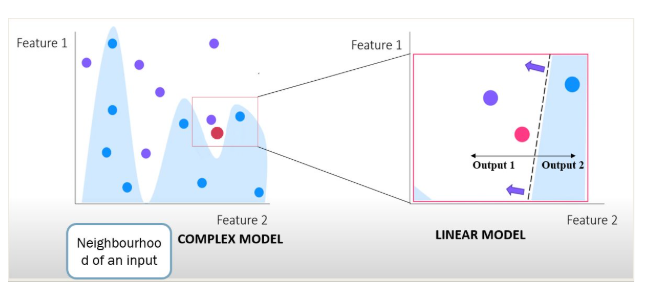
\includegraphics[width=\linewidth]{lime-1.png}
    \caption{Original dataset with a complex, non-linear decision boundary.}
\end{figure}
In the above Figure3, we see a dataset with a complex decision boundary that cannot be easily understood or explained directly.


This figure shows the selected data point (in red) whose prediction we want to explain. A local neighborhood around this point is identified using a similarity or distance function (e.g., Euclidean distance).

\begin{figure}[h]
    \centering
    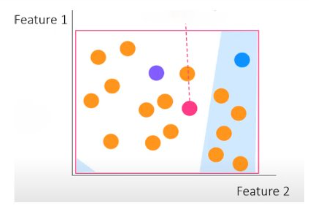
\includegraphics[width=\linewidth]{lime-2.png}
    \caption{Perturbed local neighborhood shown in orange}
\end{figure}

Finally, the neighborhood is perturbed by creating new samples as shown in Figure4, and the original model's predictions on these samples are collected. A simple interpretable model (e.g., linear regression) is then fit on these weighted samples to approximate the original model's behavior around the red point. This surrogate model provides feature importance scores that help explain the original prediction.

\subsection*{SHAP (SHapley Additive exPlanations)}

SHAP is a game-theoretic approach to explain the output of any machine learning model. It connects ideas from cooperative game theory with local explanations. The method assigns an importance value (called the Shapley value) to each feature for a particular prediction.

\subsubsection*{Shapley Values from Cooperative Game Theory}

Suppose we have a game where:
\begin{itemize}
    \item The ``players'' are the input features.
    \item The ``payout'' is the prediction \( f(x) \) from the model.
    \item The ``value function'' \( v(S) \) denotes the contribution of a subset of features \( S \subseteq F \).
\end{itemize}

The Shapley value for a feature \( i \) is defined as:

\[
\phi_i(f, x) = \sum_{S \subseteq F \setminus \{i\}} \frac{|S|!(|F| - |S| - 1)!}{|F|!} \left[ f_{S \cup \{i\}}(x) - f_S(x) \right]
\]

Where:
\begin{itemize}
    \item \( F \) is the full set of features.
    \item \( S \subseteq F \setminus \{i\} \) is a subset of features not including \( i \).
    \item \( f_S(x) \) is the expected prediction when only the features in subset \( S \) are known.
    \item The term \( f_{S \cup \{i\}}(x) - f_S(x) \) is the marginal contribution of feature \( i \) when added to subset \( S \).
\end{itemize}

\subsubsection*{SHAP in Machine Learning}

In SHAP, the prediction of a model is decomposed as:

\[
f(x) = \phi_0 + \sum_{i=1}^{M} \phi_i
\]

Where:
\begin{itemize}
    \item \( \phi_0 \) is the expected model prediction (i.e., the average over all data points).
    \item \( \phi_i \) is the Shapley value for feature \( i \), indicating how much \( i \) contributes to deviating from the expected prediction.
\end{itemize}
Using the shapley values, we select top 5 features which are most releavant for the model.

\section{Model optimisation using TinyML}
Traditional Deep Learning models often encounter limitations such as large size, computational complexity, and high energy consumption. These factors make them less suitable for deployment on resource-constrained IoT end devices. A common approach to mitigate this issue is offloading complex computational tasks from sensor nodes to edge gateways.

 However, this method may not always be efficient, as the energy required to transmit data between devices can exceed the energy used to run an ML model on the device itself.

In response to these challenges, TinyML has emerged as a specialized field focused on optimizing ML models for deployment on IoT end devices with limited resources.

\subsection{Quantization}

Quantization is a technique that reduces both the model size and computational cost by converting high-precision floating-point numbers into lower-precision formats, such as 8-bit integers. This enables faster inference and more efficient deployment, especially on resource-constrained devices like edge devices and IoT systems. The process can be compared to compressing a high-resolution image into a lower-resolution one: while some details may be lost, the result is much smaller and quicker to load.

However, this reduction in precision introduces a quantization error, which can impact model performance by creating a trade-off between size and accuracy. This error arises from the approximation of values, where certain fine-grained details are sacrificed for the sake of efficiency. Despite this trade-off, quantization remains a crucial method for optimizing machine learning models in practical, real-world applications.

\begin{figure}[h]
    \centering
    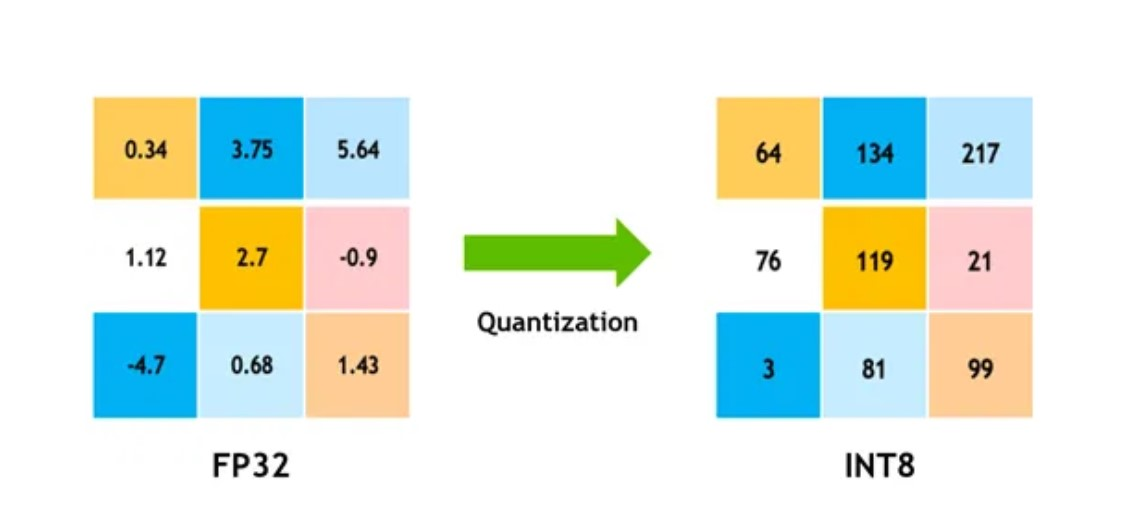
\includegraphics[width=\linewidth]{Quantized .jpg} % Replace with your actual image file name
    \caption{Illustration of the Quantization Process.} % Customize the caption as needed
    \label{fig:quantization}
\end{figure}


\subsection{Knowledge Distillation}


Knowledge Distillation (KD) transfers knowledge from a large, complex teacher model to a smaller, more efficient student model. This is particularly beneficial in resource-constrained environments, where deploying large models is impractical due to limitations in memory, processing power, and inference time.

The teacher model, typically a deep and over-parameterised network, is trained on the dataset and provides soft labels (probabilities) that guide the training of the student model. The student model, being smaller and more efficient, learns both from the true labels and the soft labels from the teacher, capturing richer data distribution information.

The distillation process minimises the difference between the teacher's and the student’s predictions using a combined loss function, which incorporates both the standard cross-entropy loss and the distillation loss. The distillation loss \( L_{KD} \) is defined as:

\[
L_{KD} = \alpha \cdot L_{\text{CE}}(y, \hat{y}) + (1 - \alpha) \cdot T^2 \cdot L_{\text{KL}}(q_{\text{teacher}}, q_{\text{student}})
\]

Where:
- \( L_{\text{CE}}(y, \hat{y}) \) is the cross-entropy loss between the true labels \( y \) and the student’s predictions \( \hat{y} \),
- \( L_{\text{KL}}(q_{\text{teacher}}, q_{\text{student}}) \) is the Kullback-Leibler divergence between the teacher’s and student’s probability distributions,
- \( T \) is the temperature parameter that smooths the soft labels for better learning by the student,
- \( \alpha \) is a balancing factor between the true labels and the soft labels.

The teacher’s output \( q_{\text{teacher}} \) and the student’s output \( q_{\text{student}} \) are computed as:

\[
q_{\text{teacher}} = \frac{\exp(z_{\text{teacher}} / T)}{\sum_j \exp(z_{\text{teacher}}^j / T)}
\]

\[
q_{\text{student}} = \frac{\exp(z_{\text{student}} / T)}{\sum_j \exp(z_{\text{student}}^j / T)}
\]

By minimizing this loss, the student model mimics the teacher’s behavior while being more computationally efficient. This approach significantly enhances the performance of small models, making them viable for deployment in real-world, resource-limited scenarios.

\begin{figure}[h]
    \centering
    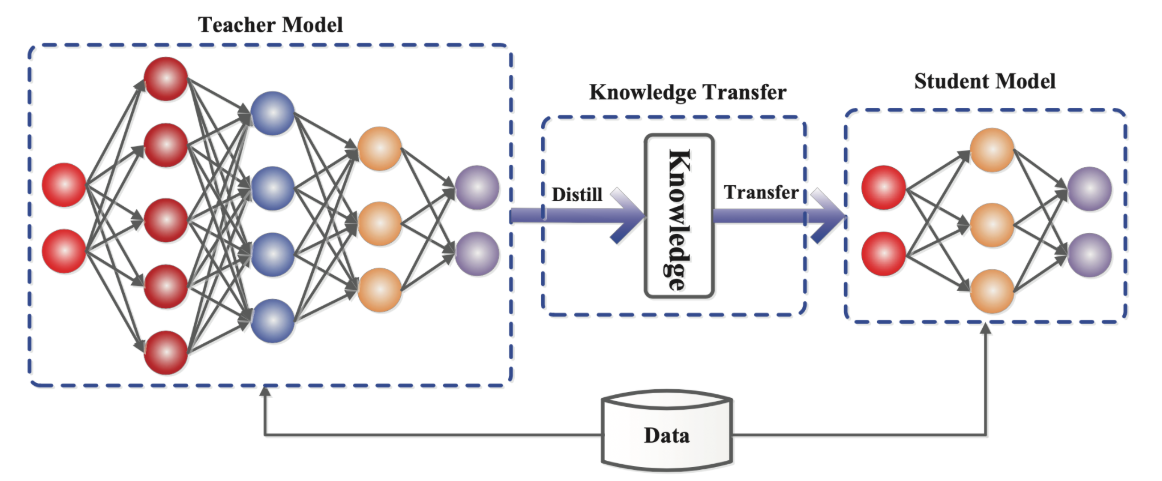
\includegraphics[width=\linewidth]{knowledge distillation .png} % Replace with your image filename
    \caption{Illustration of Knowledge Distillation Process.} % Customize the caption
    \label{fig:knowledge-distillation}
\end{figure}

\section{Experimental Setup}

We compare the performance of our work with that of the base paper on different platforms, including cloud, edge, and IoT devices. The setup includes varying hardware configurations, as summarized in Table \ref{tab:experiment-comparison}.

% \begin{table}[h!]
% \centering
% \resizebox{\columnwidth}{!}{ 
% \begin{tabular}{|c|c|c|}
% \hline
% \textbf{Platform} & \textbf{Base Paper} & \textbf{Our Work} \\
% \hline
% \textbf{Cloud} & Azure Cloud (32GB RAM) & Google Colab (12GB RAM) \\
% \hline
% \textbf{Edge} & Dell Laptop (i7-9750H, 16GB RAM) & HP Laptop (i5, 16GB RAM) \\
% \hline
% \textbf{IoT Device} & Raspberry Pi 4 (8GB RAM) & Raspberry Pi 4 (8GB RAM) \\
% \hline
% \textbf{IoT End Device} & STM32F412 (256KB RAM) & Arduino Nano 33 (256KB RAM) \\
% \hline
% \end{tabular}
% }
% \caption{Experimental Comparison Setup}
% \label{tab:experiment-comparison}
% \end{table}

\begin{table}[h!]
\renewcommand{\arraystretch}{1.0} % Increase vertical space between rows
\centering

\begin{tabular}
{|p{2.0cm}|p{2.6cm}|p{2.6cm}|}
\hline
\textbf{Platform} & \textbf{Base Paper \cite{basepaper2}} & \textbf{Our Work} \\
\hline
\textbf{Cloud} & Azure Cloud (32GB RAM) & Google Colab (12GB RAM) \\
\hline
\textbf{Edge} & Dell Laptop (i7-9750H, 16GB RAM) & HP Laptop (i5, 16GB RAM) \\
\hline
\textbf{IoT Device} & Raspberry Pi 4 (8GB RAM) & Raspberry Pi 4 (8GB RAM) \\
\hline
\textbf{IoT End Device} & STM32F412 (256KB RAM) & Arduino Nano 33 (256KB RAM) \\
\hline
\end{tabular}
\caption{Experimental Comparison Setup}
\label{tab:experiment-comparison}
\end{table}


\section{Results and Observations}
\subsection{XAI for feature selection}
\begin{figure}[H]
    \centering
    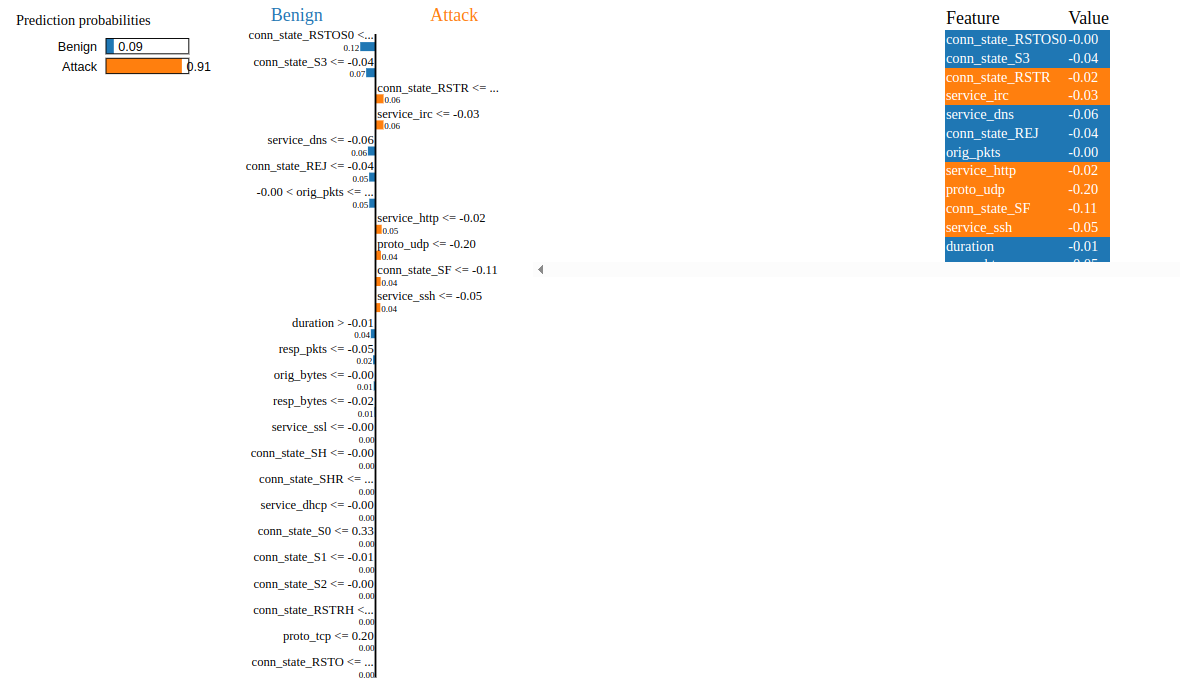
\includegraphics[width=\linewidth]{lime-result-1.png}
    \caption{LIME explanations}
    \label{fig:lime_res}
\end{figure}
The figure \ref{fig:lime_res} shows LIME Explanations. The features shown in blue colour influences Benign class and features shown in orange influences Malign class. 

\begin{figure}[h]
    \centering
    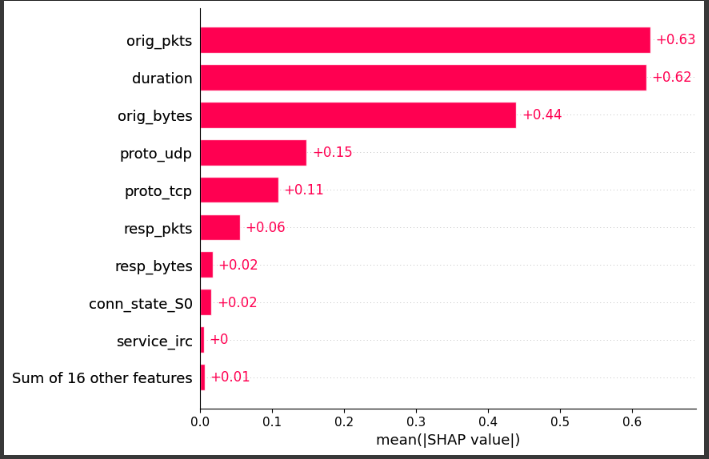
\includegraphics[width=\linewidth]{shap-result-2.png}
    \caption{SHAP explanations}
    \label{fig:shap_result}
\end{figure}
The figure \ref{fig:shap_result} shows the SHAP explanations. Using SHAP, we have identified orig\_pkts, duration, orig\_bytes, proto\_udp, proto\_tcp as the most important features. Figure 7 and figure 8 shows the effect of feature selection over accuracy and size respectively. 

\subsection{Feature Selection results}
\begin{figure}[h]
    \centering
    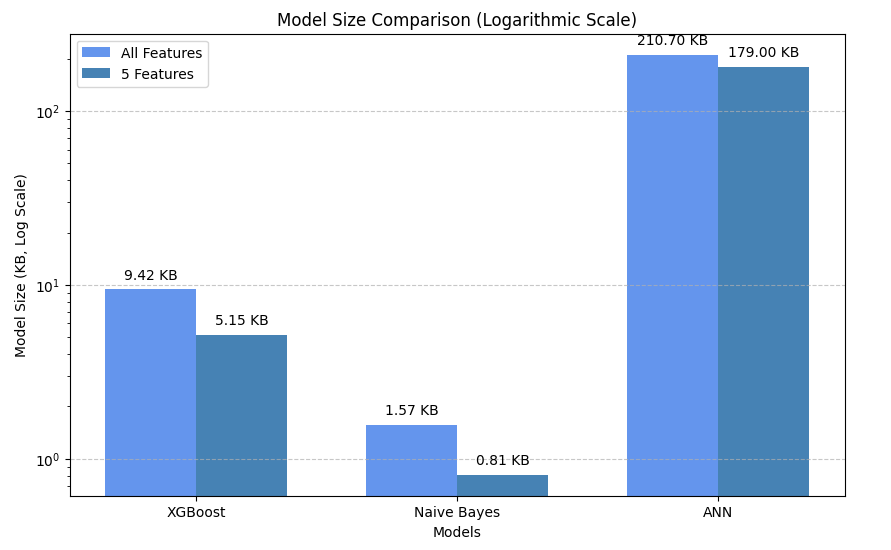
\includegraphics[width=\linewidth]{effect_FS_over_accuracy.png}
    \caption{Effect of feature selection over accuracy}
    \label{fig:fs_acc}
\end{figure}
\begin{figure}[h]
    \centering
    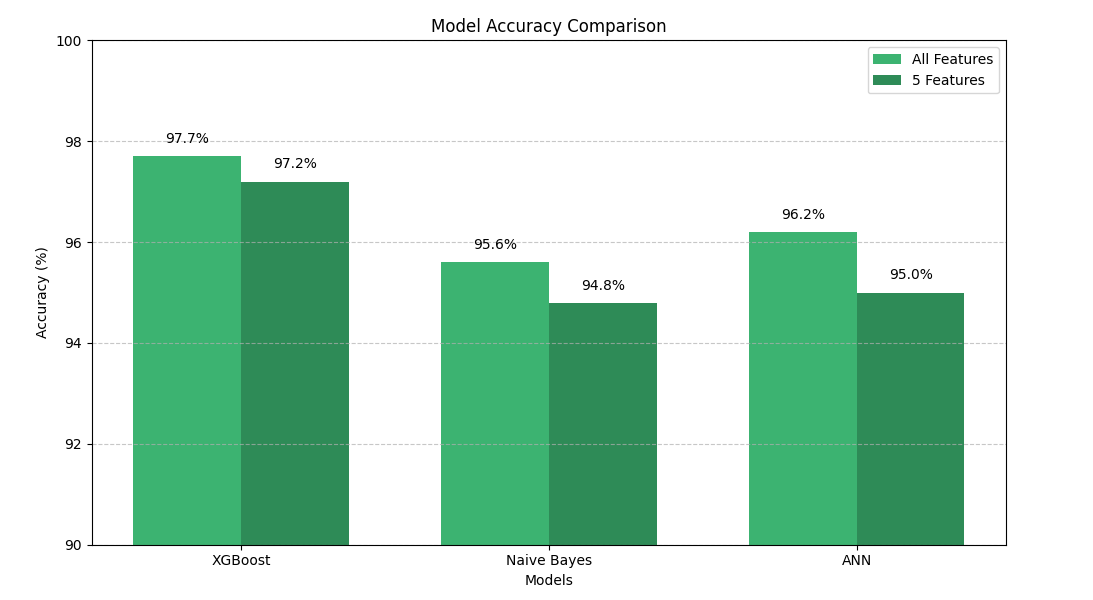
\includegraphics[width=\linewidth]{effect_FS_over_size.png}
    \caption{Effect of feature selection over size}
    \label{fig:fs_size}
\end{figure}
By performing feature selection, there is 0.5\%,0.8\% and 1.2\% accuracy loss respectively for XGB, Naive Bayes and Artificial Neural Network (ANN). On the other hand, XGB's size has been reduced to 5.15KB from 9.42KB whereas NB's size has been reduced from 0.81kB from 1.57KB. ANN's size has been reduced from 210KB to 179KB. ANN showed the least reduction in model size along with highest accuracy loss among all models. 

\subsection{Quantization Results}
\begin{figure}[h]
    \centering
    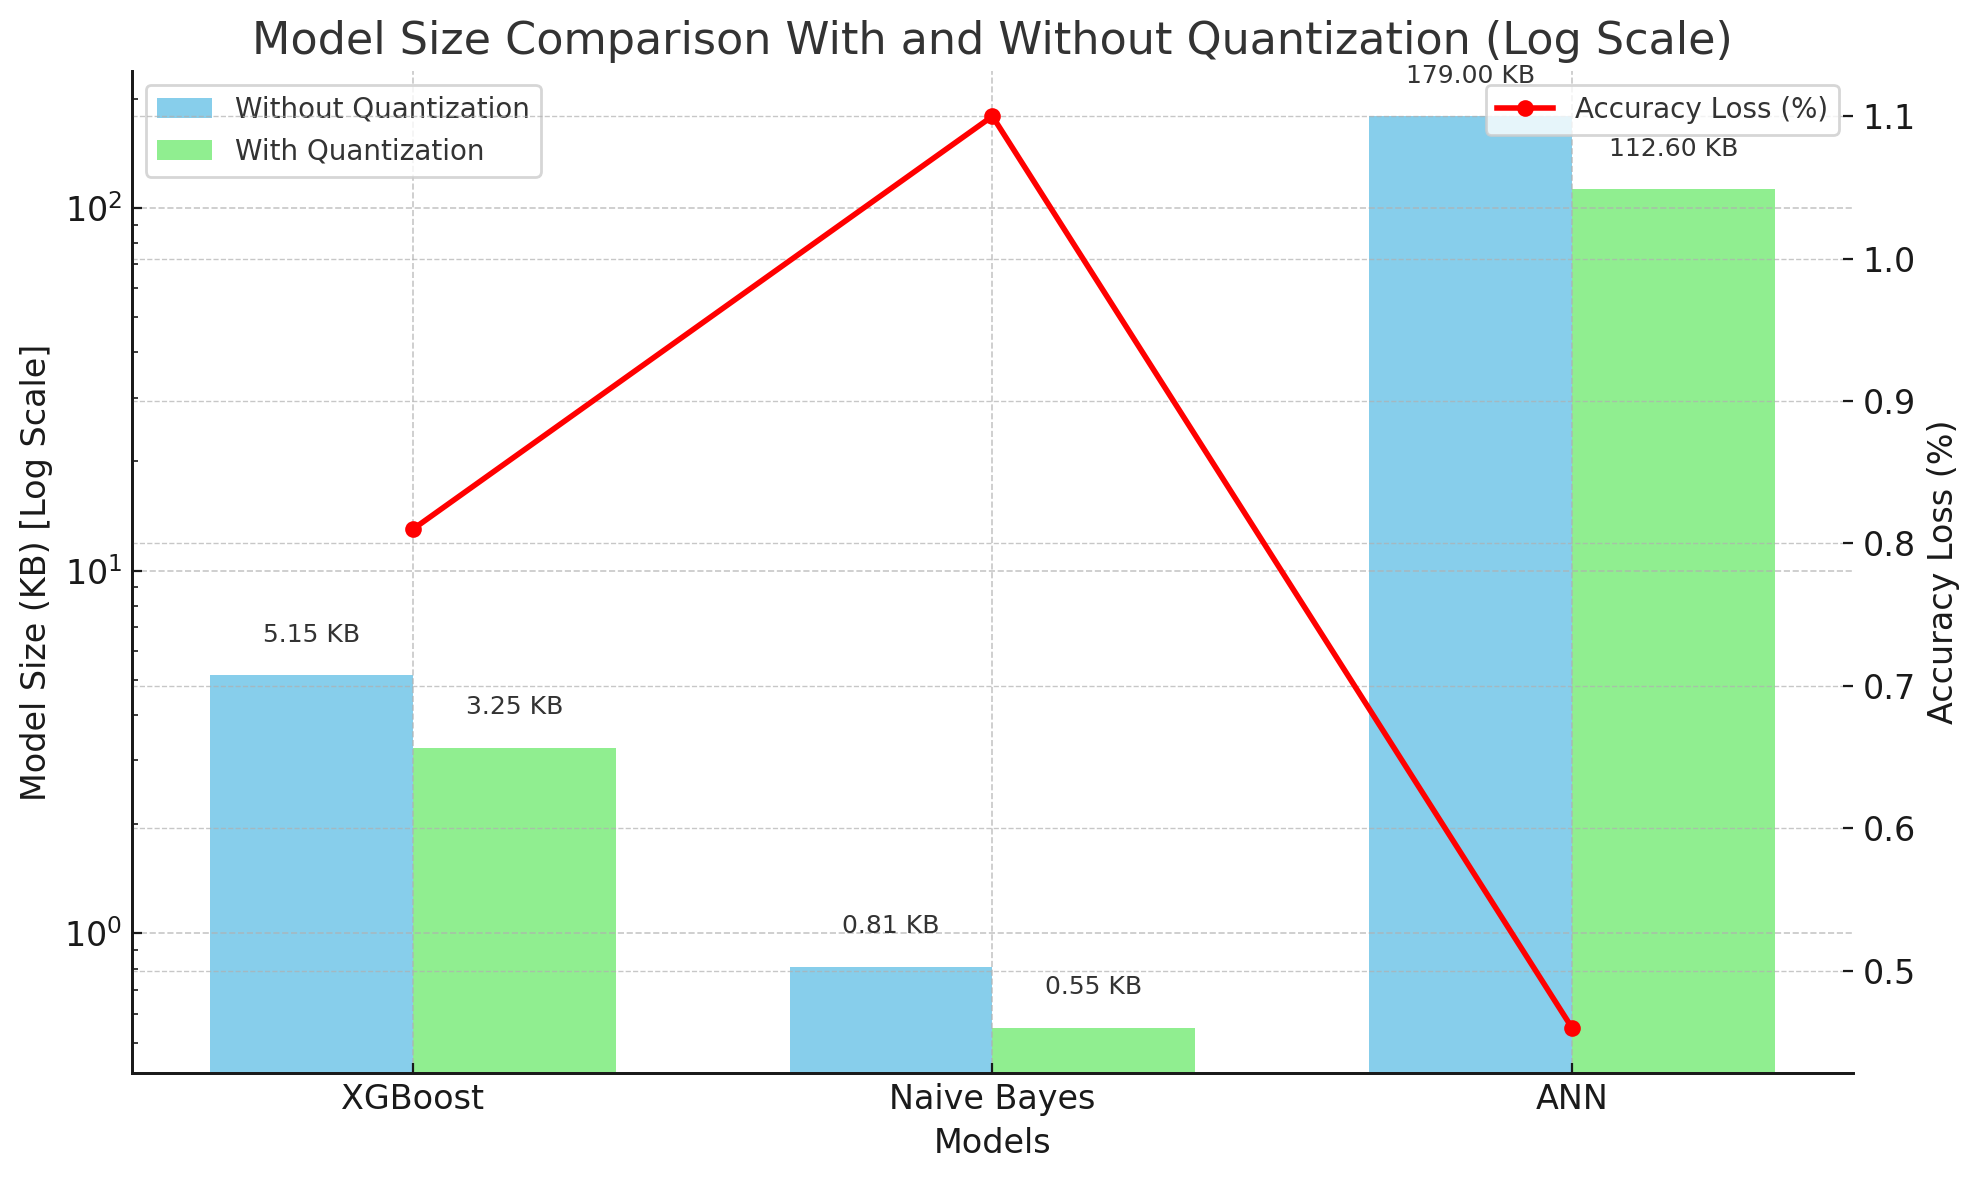
\includegraphics[width=\linewidth]{1e2800d7-96cd-42c0-9a1b-3bbc28a2501c.png}
    \caption{Effect of Quantization along with accuracy loss}
    \label{fig:quant}
\end{figure}
By performing quantization as mentioned in figure \ref{fig:quant}, we have observed 36\% , 32\%, 37\% reduction in model size (after feature selection) with 0.8\%,1.1\% and 0.3\% accuracy loss for XGB,NB and ANN respectively. This is not desired in a real-life scenario where model sizes may reach upto MBs. 

\subsection{Knowledge Distillation Results}
\begin{figure}[h]
    \centering
    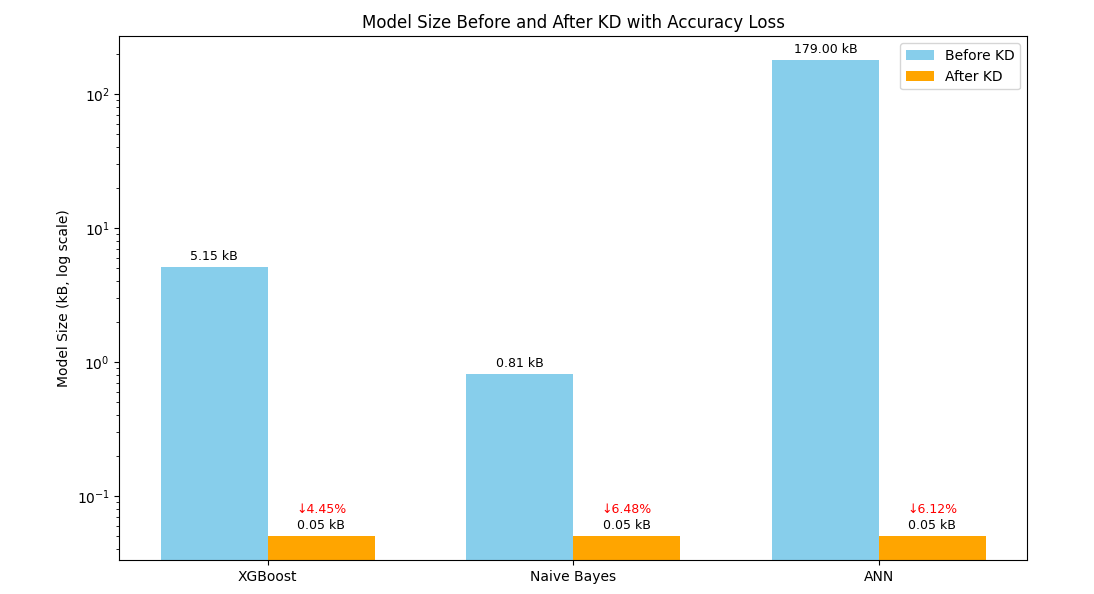
\includegraphics[width=\linewidth]{knowledge_distillation.png}
    \caption{Effect of Knowledge Distillation along with accuracy loss}
    \label{fig:fs_size}
\end{figure}
For each of the teacher models (XGB,NB,ANN), we have performed knowledge distillation to a simpler student (Logistic Regression). Hence we can observe all the student models sizes are equal to 0.05KB as mentioned in Figure 11. But training is dependent on teacher also, hence we can observe differnet accuracy losses for different cases. XGB teacher provides the minimal accuracy loss to its student while NB provides maximal accuracy loss to its student.

\subsection{Comparison with State of the Art Techniques}
\subsubsection{Training Time}
\begin{figure}[H]
    \centering
    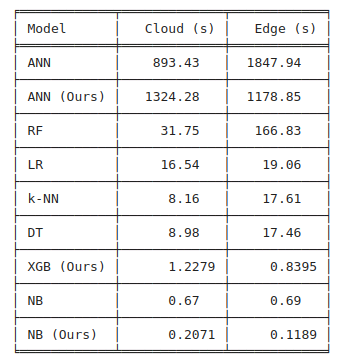
\includegraphics[width=\linewidth,height=4cm]{training.png}
    \caption{Comparison of training times with Tekin et al.}
    \label{fig:fs_size}
\end{figure}
Training times were only compared on Cloud and Edge. Our method achieves better training time compared to base paper \cite{basepaper2}.

\subsubsection{Inference Time}
\begin{figure}[H]
    \centering
    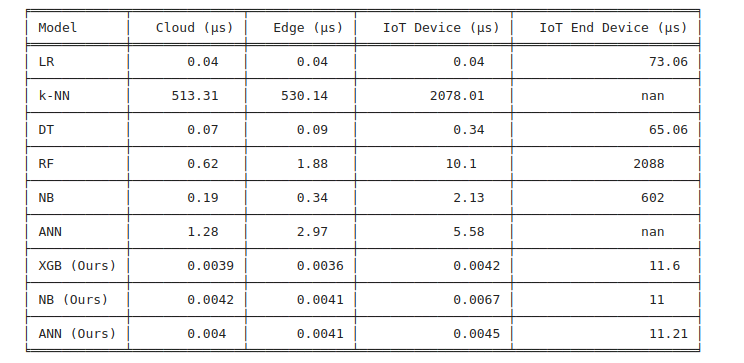
\includegraphics[width=\linewidth,height=4cm]{inference.png}
    \caption{Comparison of inference times with Tekin et al. }
    \label{fig:inferenceT}
\end{figure}
We have used Edge Impulse to simulate the working of models on IoT device and IoT end device. 
Inference times for different models are mentioned in table \ref{fig:inferenceT}. Our model surpasses \cite{basepaper2} in terms of inference times. Our best inference time on IoT end device is 11 micro seconds compared to 76 micro seconds in \cite{basepaper2}

\subsubsection{Energy consumption}
\begin{figure}[H]
    \centering
    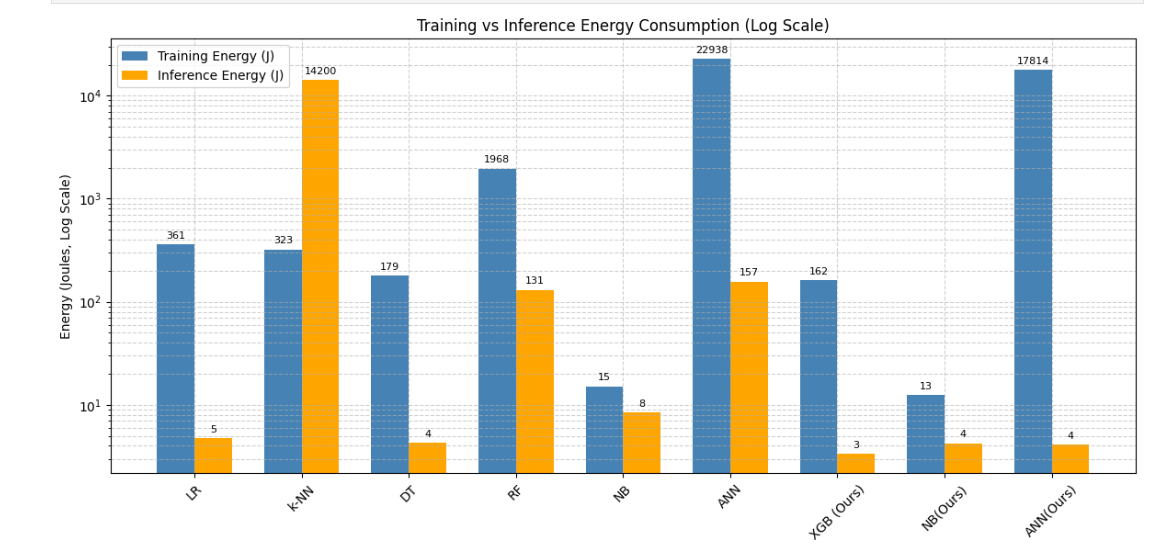
\includegraphics[width=\linewidth,height=4cm]{energy-2.png}
    \caption{Comparison of energy consumption with Tekin et al. }
    \label{fig:inferenceT}
\end{figure}
To measure energy consumption, we used Intel's RAPL(Running Average Power Limit). We have made 2 check points. One before using the model for training/inference and then after using the model for training/inference. The difference in checkpoints energy consumption revealed actual energy consumption for the process. We made sure no background apps were running during training/inference to make proper measurements.

\section{Conclusion}
In this work, we proposed a compact, explainable intrusion detection framework tailored for resource-constrained IoT environments by integrating Explainable Artificial Intelligence (XAI) with Tiny Machine Learning (TinyML). Through the use of LIME and SHAP, we performed informed feature selection, reducing the original 26 input features down to just 5 high-impact features. This significantly enhanced both model interpretability and efficiency.
\\

To ensure real-time deployability on edge devices, we incorporated quantization and knowledge distillation. These methods led to a dramatic reduction in model complexity: our initial Artificial Neural Network (ANN) with 48,800 parameters was successfully distilled into a lightweight Logistic Regression model with just 6 parameters—a 99.98\% reduction in size. Quantization further improved compactness by up to 1.4×, resulting in faster inference, lower memory usage, and reduced power consumption.

Despite this aggressive compression, our models maintained high accuracy and consistent performance on edge platforms such as Raspberry Pi 4 and Arduino Nano 33, simulated via the Edge Impulse platform.
\\

These results demonstrate that XAI-driven TinyML offers a viable path toward secure, efficient, and interpretable intrusion detection in IoT ecosystems. Future work will explore dynamic adaptation to emerging threats through incremental learning and further innovations in ultra-compact model design for even more constrained environments.
\section{Future Scope}
The journey toward building the most efficient and reliable intrusion detection system for IoT devices doesn’t stop here. While our current framework has demonstrated the power of XAI-driven feature selection and model compression through TinyML techniques, it opens the door to even more exciting advancements. As IoT ecosystems continue to grow in complexity and scale, so too must our models evolve. The following directions outline promising avenues for pushing the boundaries of adaptability, compactness, and intelligence in real-world deployments.

\subsection{Enhanced Accuracy-Compactness Trade-off}Investigate more advanced optimization techniques to further reduce model size and complexity while minimizing the impact on accuracy. Techniques like pruning, low-rank approximation, and quantization-aware training could be explored for deeper model compression.

\subsection{Incremental and Continual Learning} Develop incremental learning mechanisms that allow the model to adapt in real time to new types of attacks without requiring complete retraining. This is crucial for maintaining relevance in dynamic IoT threat landscapes.
\subsection{Building a Real-Time Classification Engine:}
The current setup might be limited to offline analysis. To unlock the true potential of these models, a robust backend system can be implemented. This backend can handle real-time data acquisition, seamlessly feed data to the chosen model, and deliver classification results instantaneously. This paves the way for deploying the model in real-world applications, enabling on-the-fly decision making.

\subsection{Making the Models Portable:}
Deploying these models on edge devices, which are often resource-constrained, might be hindered by their current size. Here, model compression techniques come into play. By strategically pruning unnecessary connections or quantizing weights, the model size can be significantly reduced without sacrificing much accuracy. This trade-off between size and accuracy allows for deploying these powerful models on devices with limited processing power, expanding their reach and impact.
\\
\\
By exploring these avenues, we can unlock a deeper understanding of the data, improve classification accuracy, and ultimately leverage these models to solve real-world problems in a more efficient and impactful way.
\vspace{7mm}
% An example of a floating figure using the graphicx package.
% Note that \label must occur AFTER (or within) \caption.
% For figures, \caption should occur after the \includegraphics.
% Note that IEEEtran v1.7 and later has special internal code that
% is designed to preserve the operation of \label within \caption
% even when the captionsoff option is in effect. However, because
% of issues like this, it may be the safest practice to put all your
% \label just after \caption rather than within \caption{}.
%
% \begin{figure}[!t]
% \centering
% \includegraphics[width=2.5in]{myfigure}
% where an .eps filename suffix will be assumed under latex, 
% and a .pdf suffix will be assumed for pdflatex; or what has been declared
% via \DeclareGraphicsExtensions.
% \caption{Simulation Results}
% \label{fig_sim}
% \end{figure}

% Note that IEEE typically puts floats only at the top, even when this
% results in a large percentage of a column being occupied by floats.


% An example of a double column floating figure using two subfigures.
% (The subfig.sty package must be loaded for this to work.)
% The subfigure \label commands are set within each subfloat command, the
% \label for the overall figure must come after \caption.
% \hfil must be used as a separator to get equal spacing.
% The subfigure.sty package works much the same way, except \subfigure is
% used instead of \subfloat.
%
%\begin{figure*}[!t]
%\centerline{\subfloat[Case I]\includegraphics[width=2.5in]{subfigcase1}%
%\label{fig_first_case}}
%\hfil
%\subfloat[Case II]{\includegraphics[width=2.5in]{subfigcase2}%
%\label{fig_second_case}}}
%\caption{Simulation results}
%\label{fig_sim}
%\end{figure*}
%
% Note that often IEEE papers with subfigures do not employ subfigure
% captions (using the optional argument to \subfloat), but instead will
% reference/describe all of them (a), (b), etc., within the main caption.


% An example of a floating 
%. Note that, for IEEE style tables, the 
% \caption command should come BEFORE the table. Table text will default to
% \footnotesize as IEEE normally uses this smaller font for tables.
% The \label must come after \caption as always.
%
%\begin{table}[!t]
%% increase table row spacing, adjust to taste
%\renewcommand{\arraystretch}{1.3}
% if using array.sty, it might be a good idea to tweak the value of
% \extrarowheight as needed to properly center the text within the cells
%\caption{An Example of a Table}
%\label{table_example}
%\centering
%% Some packages, such as MDW tools, offer better commands for making tables
%% than the plain LaTeX2e tabular which is used here.
%\begin{tabular}{|c||c|}
%\hline
%One & Two\\
%\hline
%Three & Four\\
%\hline
%\end{tabular}
%\end{table}


% Note that IEEE does not put floats in the very first column - or typically
% anywhere on the first page for that matter. Also, in-text middle ("here")
% positioning is not used. Most IEEE journals/conferences use top floats
% exclusively. Note that, LaTeX2e, unlike IEEE journals/conferences, places
% footnotes above bottom floats. This can be corrected via the \fnbelowfloat
% command of the stfloats package.



% trigger a \newpage just before the given reference
% number - used to balance the columns on the last page
% adjust value as needed - may need to be readjusted if
% the document is modified later
%\IEEEtriggeratref{8}
% The "triggered" command can be changed if desired:
%\IEEEtriggercmd{\enlargethispage{-5in}}

% references section

% can use a bibliography generated by BibTeX as a .bbl file
% BibTeX documentation can be easily obtained at:
% http://www.ctan.org/tex-archive/biblio/bibtex/contrib/doc/
% The IEEEtran BibTeX style support page is at:
% http://www.michaelshell.org/tex/ieeetran/bibtex/
% argument is your BibTeX string definitions and bibliography database(s)
\bibliography{biblio}
\bibliographystyle{IEEEtran}

\end{document}
%%%%%%%%%%%%%%%%%%%%%%%%%%%%%%%%%%%%%%%%%%%%%%%%%%%%%%%%%%%%%%%%%%%%%%%
%% STUFF FROM THE TOP
%% bare_conf.tex
%% V1.3
%% 2007/01/11
%% by Michael Shell
%% See:
%% http://www.michaelshell.org/
%% for current contact information.
%%
%% This is a skeleton file demonstrating the use of IEEEtran.cls
%% (requires IEEEtran.cls version 1.7 or later) with an IEEE conference paper.
%%
%% Support sites:
%% http://www.michaelshell.org/tex/ieeetran/
%% http://www.ctan.org/tex-archive/macros/latex/contrib/IEEEtran/
%% and
%% http://www.ieee.org/

%%*************************************************************************
%% Legal Notice:
%% This code is offered as-is without any warranty either expressed or
%% implied; without even the implied warranty of MERCHANTABILITY or
%% FITNESS FOR A PARTICULAR PURPOSE! 
%% User assumes all risk.
%% In no event shall IEEE or any contributor to this code be liable for
%% any damages or losses, including, but not limited to, incidental,
%% consequential, or any other damages, resulting from the use or misuse
%% of any information contained here.
%%
%% All comments are the opinions of their respective authors and are not
%% necessarily endorsed by the IEEE.
%%
%% This work is distributed under the LaTeX Project Public License (LPPL)
%% ( http://www.latex-project.org/ ) version 1.3, and may be freely used,
%% distributed and modified. A copy of the LPPL, version 1.3, is included
%% in the base LaTeX documentation of all distributions of LaTeX released
%% 2003/12/01 or later.
%% Retain all contribution notices and credits.
%% ** Modified files should be clearly indicated as such, including  **
%% ** renaming them and changing author support contact information. **
%%
%% File list of work: IEEEtran.cls, IEEEtran_HOWTO.pdf, bare_adv.tex,
%%                    bare_conf.tex, bare_jrnl.tex, bare_jrnl_compsoc.tex
%%*************************************************************************